\documentclass{beamer}
\usetheme{Madrid}
\usecolortheme{default}
\usepackage{listings}
\usepackage{tcolorbox}
\usepackage{booktabs}
\tcbuselibrary{listings, skins}

\newtcblisting{mycode}{
  arc=0mm,                          % Sharp corners
  boxrule=0.5pt,                    % Border thickness
  colback=white,                    % Background color
  colframe=black,                   % Border color
  listing only, 
  listing options={
    language=Python,
    basicstyle=\small\ttfamily,      % Monospace font
    keywordstyle=\color{blue},       % Color for 'import', etc.
    commentstyle=\color{blue},       % Color for comments
    stringstyle=\color{red},
    showstringspaces=false,
    breaklines=true
  },
  sharp corners,
  enhanced,
}

\title{Discrete-2.0.27}
\author{INDHIRESH S-EE25BTECH11027}
\date{\today}

\begin{document}

\begin{frame}
    \titlepage
\end{frame}

\begin{frame}{Question}
 A point on a curve is said to be an extremum if it is a local minimum or a local maximum. The number of distinct extrema for the curve $3x^4 -16x^3 + 24x^2 + 37 $ is

\begin{columns}[t]
    \begin{column}{0.45\textwidth}
        \begin{enumerate}[a)]
            \item 0
            \item 1
        \end{enumerate}
    \end{column}
    
    \begin{column}{0.45\textwidth}
        \begin{enumerate}[a)]
            \setcounter{enumi}{2} % Starts the count at 'c'
            \item 2
            \item 3
        \end{enumerate}
    \end{column}
\end{columns}
\end{frame}



\begin{frame}{Problem Overview}
    \begin{block}{The Question}
        Determine the number of distinct extrema for the curve:
        \[ f(x) = 3x^4 - 16x^3 + 24x^2 + 37 \]
    \end{block}
    
    \begin{itemize}
        \item \textbf{Extremum:} A point that is either a local maximum or a local minimum.
        \item \textbf{Strategy:}
        \begin{enumerate}
            \item Find the first derivative $f'(x)$.
            \item Identify critical points where $f'(x) = 0$.
            \item Analyze sign changes to confirm extrema.
        \end{enumerate}
    \end{itemize}
\end{frame}

% Slide 3: Calculus Step
\begin{frame}{Step 1: Finding Critical Points}
    Differentiate the function with respect to $x$:
    \[ f'(x) = 12x^3 - 48x^2 + 48x \]
    
    Set the derivative to zero to find stationary points:
    \[ 12x(x^2 - 4x + 4) = 0 \]
    \[ 12x(x - 2)^2 = 0 \]
    
    \textbf{Critical Points:}
    \begin{itemize}
        \item $x = 0$
        \item $x = 2$
    \end{itemize}
\end{frame}

% Slide 4: Testing for Extrema
\begin{frame}{Step 2: Analysis of Critical Points}
    We use the \textbf{First Derivative Test} to check for sign changes:
    
    \begin{table}[]
        \centering
        \begin{tabular}{@{}l l l l@{}}
        \toprule
        \textbf{Point} & \textbf{Interval} & \textbf{Sign of $f'(x)$} & \textbf{Behavior} \\ \midrule
        $x = 0$        & $x < 0$           & Negative ($-$)           & Decreasing        \\
                       & $x > 0$           & Positive ($+$)           & Increasing        \\ \midrule
        $x = 2$        & $x < 2$           & Positive ($+$)           & Increasing        \\
                       & $x > 2$           & Positive ($+$)           & Increasing        \\ \bottomrule
        \end{tabular}
    \end{table}

    \begin{itemize}
        \item At \textbf{$x = 0$}: Sign changes from $-$ to $+ \rightarrow$ \textbf{Local Minimum}.
        \item At \textbf{$x = 2$}: No sign change $\rightarrow$ \textbf{Inflection Point}.
    \end{itemize}
\end{frame}

% Slide 5: Conclusion
\begin{frame}{Conclusion}
    \begin{itemize}
        \item The curve has two stationary points ($x=0, 2$).
        \item Only \textbf{one} of these points ($x=0$) is an extremum.
    \end{itemize}
    
    \vspace{1cm}
    \begin{center}
        \textbf{Final Answer: (b) 1}
    \end{center}
\end{frame}


\begin{frame}[fragile]
\frametitle{Python Code for Plot}
\begin{mycode}
import sympy as sp
import numpy as np
import matplotlib.pyplot as plt

# --- Step 1: SymPy Symbolic Analysis ---
# Define the symbolic variable and function
x_sym = sp.Symbol('x')
f_sym = 3*x_sym**4 - 16*x_sym**3 + 24*x_sym**2 + 37

# Find the first derivative and critical points
f_prime = sp.diff(f_sym, x_sym)
critical_points = sp.solve(f_prime, x_sym) # Exact algebraic solutions
\end{mycode}

\end{frame}

\begin{frame}[fragile]
\frametitle{Python Code for Plot}
\begin{mycode}
# Find the second derivative for testing curvature
f_double_prime = sp.diff(f_prime, x_sym)

# Dictionaries to store categorized extrema for plotting
minima_found = []
maxima_found = []

print("--- SymPy Analysis Results ---")
print(f"Critical Points Found: {critical_points}")

for pt in critical_points:
    # 1. Find exact y-value
    y_val = f_sym.subs(x_sym, pt)
    
   
\end{mycode}

\end{frame}

\begin{frame}[fragile]
\frametitle{Python Code for Plot}
\begin{mycode}
# 2. Find curvature at point
    curvature = f_double_prime.subs(x_sym, pt)
    
    if curvature > 0:
        print(f"Point x={pt}, y={y_val} is a Local Minimum (Extremum)")
        minima_found.append((float(pt), float(y_val)))
    elif curvature < 0:
        print(f"Point x={pt}, y={y_val} is a Local Maximum (Extremum)")
        maxima_found.append((float(pt), float(y_val)))
    else:
        print(f"Point x={pt}, y={y_val} is an Inflection Point (Not an Extremum)")



\end{mycode}

\end{frame}

\begin{frame}[fragile]
\frametitle{Python Code for Plot}
\begin{mycode}
f_num = sp.lambdify(x_sym, f_sym, 'numpy')

# Generate numerical x-values (range selected to show the behavior)
x_vals = np.linspace(-1, 3.5, 400)
y_vals = f_num(x_vals)

# Setup the plot
plt.figure(figsize=(10, 6))
plt.plot(x_vals, y_vals, label='$f(x)$ curve', color='black', linewidth=1.5, zorder=1)



\end{mycode}

\end{frame}
\begin{frame}[fragile]
\frametitle{Python Code for Plot}
\begin{mycode}

    for mx, my in minima_found:
        plt.annotate(f'Min\n({mx:.1f}, {my:.0f})', xy=(mx, my), xytext=(mx+0.2, my-15), weight='bold', color='green')
        
if maxima_found:
    max_xs, max_ys = zip(*maxima_found)
    plt.scatter(max_xs, max_ys, color='red', marker='D', s=150, edgecolors='black', label='Local Maxima', zorder=5)
else:
    print("Note: No local maximum exists for this polynomial.")



\end{mycode}

\end{frame}
\begin{frame}[fragile]
\frametitle{Python Code for Plot}
\begin{mycode}

# Styling
plt.title('Plot', fontsize=14)
plt.xlabel('x', fontsize=12)
plt.ylabel('f(x)', fontsize=12)
plt.grid(True, linestyle='--', alpha=0.5)
plt.legend()

plt.show()

\end{mycode}

\end{frame}
\begin{frame}{Plot}
\begin{figure}[H]
    \centering
    
\includegraphics[width=\linewidth]{plot.png}
    \caption{Plot}
    \label{fig:placeholder}
\end{figure}    

\end{frame}
\begin{frame}{Sympy analysis results}
    

\begin{figure}[H]
    \centering
    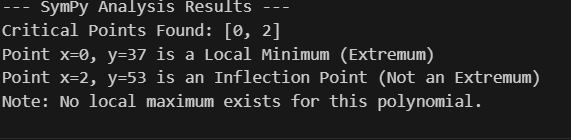
\includegraphics[width=\linewidth]{Output.png}
    \caption{Output}
    \label{fig:placeholder}
\end{figure}

\end{frame}

\end{document}